\section{Test des \acp{poc} }\label{sec:poc:test}
\subsection{Testaufbau}
Das Backend des \acp{poc} ist auf einem Computer mit dem Betriebssystem Ubuntu installiert. 
Die statischen Dokumente (\ac{js}, \ac{html} und \ac{css}) werden von einem \emph{Apache HTTP Server} \citep{apache} gehostet.
Die Datenbank ist eine MariaDB Datenbank.
Der Zugriff auf das \ac{scada} System erfolgt über ein zweiten Computer.
Verschlüsselt wird die Verbindung zwischen Frontend und Backend durch ein selbst ausgestelltes und selbstsigniertes Zertifikat.
Das Frontent wird durch den Browser \eigenName{Chrome} in der Version 77.0.3865.120 von \emph{Google LLC} ausgeführt und angezeigt.
Die \ac{opcua} Schnittstelle wird zu Testzwecken mit der Software \eigenName{UaExpert} in der Version 1.5.1 331 der \emph{Unified Automation GmbH} angesprochen.
Das Netzwerk besteht aus dem einen Computer mit dem Backend, sowie einem weiteren Computer mit Windows 7.
Auf dem Windows Computer wird die Software \eigenName{UaExpert} sowie \eigenName{Chrome} ausgeführt.
Beide Rechner sind in einem  1GBit Ethernet Netzwerk durch ein Switch verbunden.

\begin{figure}
  \centering
  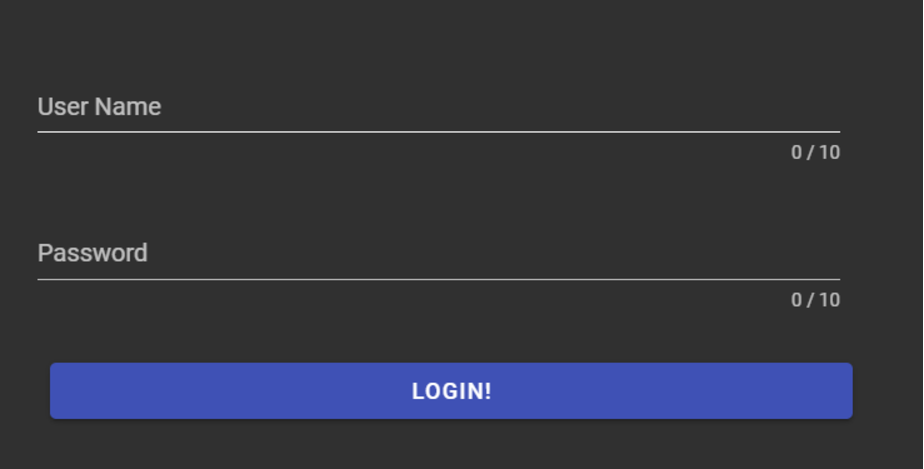
\includegraphics[width=\textwidth]{content/hauptteil/umsetzungPoC/pocTest/res/screenLogin.pdf}
  \caption{Screenshot der Login Seite}
  \label{fig:frontend:poc:login}
\end{figure}


\begin{figure}[ht]
  \centering
  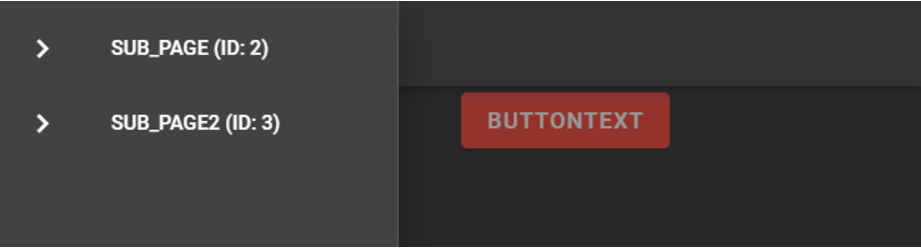
\includegraphics[width=\textwidth]{content/hauptteil/umsetzungPoC/pocTest/res/screenPageNav.pdf}
  \caption{Screenshot einer Beispielseite mit ausgeklappter Navigation}
  \label{fig:frontend:poc:nav}
\end{figure}


\begin{figure}[ht]
  \centering
  \begin{subfigure}[b]{\textwidth}
    \centering
    
\includegraphics[width=\textwidth]{content/hauptteil/umsetzungPoC/pocTest/res/screenPage.pdf}
    \caption{\emph{DataNode} \eigenName{ButtonState} = \emph{false}}
    \label{fig:frontend:poc:button:true}
  \end{subfigure}
  \hspace{50.00mm}
  \begin{subfigure}[b]{\textwidth}
      \centering
      
\includegraphics[width=\textwidth]{content/hauptteil/umsetzungPoC/pocTest/res/screenButtonClicked.pdf}
      \caption{\emph{DataNode} \eigenName{ButtonState} = \emph{false}}
      \label{fig:frontend:poc:button:false}
  \end{subfigure}
  \caption[Screenshot einer Seite mit Button]{Screenshot einer Seite mit Button in zwei verschiedenen Zuständen}
  \label{fig:frontend:poc:button}
\end{figure}